\documentclass{beamer}
\usetheme{CambridgeUS}
\usecolortheme{beaver}
\usepackage{xeCJK}
\usepackage{hyperref}

\usefonttheme[onlymath]{serif}
\begin{document} 

\begin{frame}
    \title{生生函数的运算与组合计数问题} 
    \begin{titlepage}
    \end{titlepage}
\end{frame} 

\section{生成函数} 

\begin{frame}{生成函数是啥}
    \begin{itemize}
        \item 想必大家已经很熟练了
        \item 对于数列$\{a_i\}$,我们定义它的普通生成函数(OGF)和指数生成函数(EGF)分别为
        $$\begin{aligned}
            A(x) &= \sum_{i\geq 0} a_i x^i\\
            \hat A(x) &= \sum_{i\geq 0} a_i \frac{x^i}{i!}
        \end{aligned}$$\pause
        \item 普通生成函数解决无标号问题,指数生成函数解决有标号问题
    \end{itemize}
\end{frame}

\begin{frame}{生成函数是啥}
    \begin{itemize}
        \item 两个普通生成函数的乘积$A(x)\times B(x)$可以理解为,从$A$中选择一个元素,再从$B$中选取一个元素,然后再将它们拼接起来\pause
        \item 比如说,有两个不相同的骰子,问有多少种方式使得两个骰子朝上的点数之和为8\pause
        \item 答案的生成函数为$(x + x^2 + x^3 + x^4 + x^5 + x^6)^2$
    \end{itemize}
\end{frame}

\begin{frame}{生成函数是啥}
    \begin{itemize}
        \item 两个指数生成函数的乘积$\hat A(x)\times \hat B(x)$可以理解为,$\hat A$中的元素内部已经分配好了编号,$\hat B$中的元素也已经分配好了编号。现在要将这两个序列中的元素组合起来,并且重新分配编号,且不能改变$\hat A,\hat B$中编号大小的相对顺序\pause
        $$\begin{aligned}
            \hat C(x) &= \hat A(x)\times \hat B(x)\\
            \frac{C_n}{n!} &= \sum_{i + j = n}\frac{A_i}{i!}\times \frac{B_j}{j!}\\
            C_n &= \sum_{i + j = n}A_i\times B_j\times {i + j\choose i}
        \end{aligned}$$
    \end{itemize}
\end{frame}

\begin{frame}{非常小的练习(我找不到题了)}
    \begin{itemize}
        \item 为了保证大家都在线,这里有两个简单的小练习
        \item 设$a_n$表示将$n$个完全相同的球放入编号为$1\sim 5$的篮子的方案数,其中编号为$1,2$的篮子中的球数必须是偶数,剩下的三个篮子每个篮子中的球数必须介于$3\sim 5$之间,求$a_n$的OGF
        \item 设$a_n$表示将$n$个不同的球放入$k$个不同的盒子的方案数,盒子可以是空的,求$a_n$的EGF
    \end{itemize}
\end{frame}

\begin{frame}{非常重要的展开式}
    \begin{itemize}
        \item 二项式定理
        \item $1 + x + x^2 + x^3 + \cdots = \frac{1}{1 - x}$
        \item $x + \frac{x^2}{2} + \frac{x^3}{3} + \cdots = -\ln(1 - x)$
        \item $1 + x + \frac{x^2}{2!} + \frac{x^3}{3!} + \cdots = \exp(x)$
    \end{itemize}
\end{frame}

\begin{frame}{多项式求逆}
    \begin{block}{问题}
        已知$A(x)\times B(x) \equiv 1\pmod {x^n}$,给出$A(x)$,求$B(x)$\newline
        保证$A_0\neq 0$
    \end{block} \pause
    \begin{itemize}
        \item 假设已经求出了$B'(x)$满足$A(x)\times B'(x)\equiv 1\pmod {x^{\lceil\frac n2\rceil}}$\pause
        $$\begin{aligned}
            A(x)\times B(x)&\equiv 1\pmod {x^{\lceil\frac n2\rceil}}\\ 
            \Rightarrow B(x)&\equiv B'(x) \pmod {x^{\lceil\frac n2\rceil}}\\ \pause
            B(x)^2 - 2B(x)B'(x) + B'(x)^2 &\equiv 0\pmod {x^n}\\ \pause
            B(x) - 2B'(x) + B'(x)^2A(x) &\equiv 0\pmod{x^n}\\
            2B'(x) - B'(x)^2A(x) &\equiv B(x)\pmod{x^n} 
        \end{aligned}$$
    \end{itemize}
\end{frame}

\begin{frame}{多项式$\ln$}
    \begin{block}{问题}
        已知$A(x)\equiv \ln B(x) \pmod {x^n}$,给出$B(x)$,求$A(x)$
    \end{block} \pause
    \begin{itemize}
        \item 相信大家都没有忘记小学三年级教的求导和积分 \pause
        $$\begin{aligned}
            A'(x) &= \frac{B'(x)}{B(x)}
        \end{aligned}$$ \pause
        \item 对$B(x)$求逆之后做一次NTT,再积分回去即可科技为了你
    \end{itemize}
\end{frame}

\begin{frame}{关于泰勒展开}
    \begin{itemize}
        \item 将多项式$F(x)$展开为无穷级数的形式 \pause
        \item 每一个$F(x)$,都有其唯一确定的导函数$F'(x)$ 
        \item 比如$F(x) = x^3 + 3$,我们可以得到$F'(x) = 3x^2$ \pause
        \item 但是我们不能逆用这个过程,因为有很多函数的导函数都是$F'(x) = 3x^2$,具体来说,这类函数是$F(x) = x^3 + C$ \pause
        \item 有一句话说得很好:原函数的信息=导函数的信息+初始值信息 \pause
    \end{itemize}
\end{frame}

\begin{frame}{关于泰勒展开}
    \begin{itemize}
        \item 我们选择一个点$x_0$来获取$F(x)$的初始值信息,我们将$x_0$称为展开点 \pause
        \item 接下来考虑$x_0 = 0$的情况 \pause
        $$\begin{aligned}
            F(x) &= \int_{0}^x F'(x) \,\mathrm{d}x + F(0)\\
            &= \int_{0}^x \left[\int_{0}^x F''(x) \,\mathrm{d}x + F'(0)\right] \,\mathrm{d}x + F(0)\\
            &= \int_{0}^x \int_{0}^x F''(x) \,\mathrm{d}x \,\mathrm{d}x + \int_{0}^x F'(0) \,\mathrm{d}x + F(0)
        \end{aligned}$$
    \end{itemize}
\end{frame}

\begin{frame}{多来几项}
    \begin{itemize}
        \item 可以发现最终$F(x)$被展开成了如下的形式 \pause
        $$\begin{aligned}
            F(x) &= F(0) + \int_{0}^x F'(0) \,\mathrm{d}x + \int_{0}^x \int_{0}^x F''(0) \,\mathrm{d}x\,\mathrm{d}x + \cdots\\
            &= F(0) + \frac{F'(0)x}{1} + \frac{F''(0)x^2}{1\times 2} + \cdots\\
            &= \sum_{i\geq 0} \frac{F^{(i)}(0)x^i}{i!}
        \end{aligned}$$
    \end{itemize}
\end{frame}

\begin{frame}{更一般的情况}
    \begin{itemize}
        \item 假如展开点不是$0$,而是$a$,该怎么办 \pause
        $$\begin{aligned}
            F(x) &= \int_{a}^x F'(x) \,\mathrm{d}x + F(a)\\
            &= F(a) + \int_{a}^x F'(a) \,\mathrm{d}x + \int_{a}^x \int_{a}^x F''(a) \,\mathrm{d}x \,\mathrm{d}x + \cdots
        \end{aligned}$$ \pause
        \item 令$u = x - a$,应用换元积分 \pause
        $$\begin{aligned}
            F(x) &= F(a) + \int_{0}^{u} F'(a) \,\mathrm{d}u + \int_{0}^{u} \int_{0}^{u} F''(a) \,\mathrm{d}u \,\mathrm{d}u + \cdots\\
            &= \sum_{i\geq 0} \frac{F^{(i)}(a)u^i}{i!} = \sum_{i\geq 0} \frac{F^{(i)}(a)(x - a)^i}{i!}
        \end{aligned}$$
    \end{itemize}
\end{frame}

\begin{frame}{牛顿迭代}
    \begin{block}{问题}
        已知$G[F(x)] \equiv 0\pmod {x^n}$,给出$G(x)$,求$F(x)$
    \end{block} \pause
    \begin{itemize}
        \item 记$F_t(x)$表示经过$t$次迭代之后的$F(x)$,满足
        $$\begin{aligned}
            G[F_t(x)] \equiv 0\pmod{x^{2^t}}
        \end{aligned}$$ \pause
        \item 考虑泰勒展开公式,对于函数$H(x)$,选择展开点$x_0$,那么有
        $$\begin{aligned}
            H(x) = \sum_{i\geq 0}\frac{H^{(i)}(x_0)}{i!}(x - x_0)^i
        \end{aligned}$$
    \end{itemize}
\end{frame}

\begin{frame}{牛顿迭代}
    \begin{itemize}
        \item 考虑将$G[F_{t+1}(x)]$从$F_t(x)$处展开 \pause
        $$\begin{aligned}
            G[F_{t+1}(x)]&=\sum_{i\geq 0}\frac{G^{(i)}[F_t(x)]}{i!}[F_{t+1}(x)-F_t(x)]^i\\ 
            &= G[F_t(x)] + G'[F_t(x)]\times [F_{t+1}(x) - F_t(x)] + \sum_{i\geq 2}\cdots\\  \pause
            0&\equiv G[F_t(x)] + G'[F_t(x)]\times [F_{t+1}(x) - F_t(x)]\pmod {x^{2^{t+1}}}\\ 
            F_{t+1}(x)&\equiv F_t(x) - \frac{G[F_t(x)]}{G'[F_t(x)]}\pmod {x^{2^{t + 1}}}
        \end{aligned}$$ \pause
        \item 注意这里的$G'[F_t(x)]$是先求出$G'(x)$,再代入$F_t(x)$,并非对$G[F_t(x)]$求导
    \end{itemize}
\end{frame}

\begin{frame}{多项式$\exp$}
    \begin{block}{问题}
        已知$A(x)\equiv \exp B(x) \pmod {x^n}$,给出$B(x)$,求$A(x)$
    \end{block} \pause
    \begin{itemize}
        \item 构造函数$G(x)$满足$G[A(x)] = 0$ \pause
        \item $G[A(x)] = \ln A(x) - B(x)$ \pause
        \item 应用牛顿迭代公式,可以得到 \pause
        $$\begin{aligned}
            G'[A(x)] &= \frac{1}{A(x)}\\
            F_{t+1}(x) &\equiv F_t(x) - \frac{G[F_t(x)]}{G'[F_t(x)]}\pmod {x^{2^{t + 1}}}\\
            &\equiv F_t(x)[1 - \ln F_t(x) + B(x)]\pmod {x^{2^{t + 1}}}
        \end{aligned}$$
    \end{itemize}
\end{frame}

\begin{frame}{来$k$道题}
    \begin{block}{经典问题}
        有若干种颜色不同的骨牌,其中大小为$1\times i$的骨牌共有$a_i$种,每种骨牌数量无限,问恰好填满$1\times n$的格子的方法。颜色相同的骨牌之间没有区别
        $$\begin{aligned}
            a_i, n\leq 10^5
        \end{aligned}$$
    \end{block}
\end{frame}

\begin{frame}{经典问题}
    \begin{itemize}
        \item 设$a$的OGF为$A(x)$,可以看出答案的OGF为
        $$\begin{aligned}
            \sum_{i\geq 0}A(x)^i=\frac{1}{1 - A(x)}
        \end{aligned}$$
        \item 非常良心
    \end{itemize}
\end{frame}

\begin{frame}{另一道经典问题}
    \begin{block}{论文中的题}
        给定集合$S$和正整数$n$,求有多少个$n$阶置换$p$,满足$p$分解之和每一个轮换的大小都在$S$内
        $$\begin{aligned}
            n\leq 10^5
        \end{aligned}$$
    \end{block}
\end{frame}

\begin{frame}{论文中的题}
    \begin{itemize}
        \item 置换与分解出的轮换一一对应\pause
        \item 假设原置换分解出的一个轮换长度为$n$,那么这个轮换中的元素一共有$(n-1)!$种排列方式\pause
        \item 原置换由若干个这样的轮换组成,且轮换与轮换之间是无序的\pause
        \item 写出一个轮换的EGF\pause
        $$\begin{aligned}
            \hat F(x) = \sum_{i\in S}(i-1)!\frac{x^i}{i!}
        \end{aligned}$$
    \end{itemize}
\end{frame}

\begin{frame}{论文中的题}
    \begin{itemize}
        \item 枚举最终的置换是由多少个轮换组成的,由于轮换是无序的,因此要除以一个阶乘\pause
        $$\begin{aligned}
            \hat G(x) = \sum_{i\geq 0}\frac{F(x)^i}{i!}
        \end{aligned}$$
        \item 喜闻乐见的$\exp$
    \end{itemize}
\end{frame}

\begin{frame}{经典问题}
    \begin{block}{论文中的题*2}
        你有若干种不同的物品,其中体积为$i$的物品有$a_i$种,每种物品有无限个。求选取物品恰好装满容量为$n$的背包的方案数
        $$n\leq 10^5$$
    \end{block}
\end{frame}

\begin{frame}{经典问题}
    \begin{itemize}
        \item 设$F(x)$是答案的OGF,$G(x)$是$\{a_i\}$的OGF \pause
        $$\begin{aligned}
            F(x)&=\prod_{i=1}^n(1+x^i+x^{2i}+x^{3i}+\cdots)^{a_i}\\
            &=\prod_{i=1}^n(\frac{1}{1-x^i})^{a_i}\\
            &=\exp\left(-\sum_{i=1}^na_i\ln(1-x^i)\right)\\
            &=\exp\left(\sum_{i=1}^na_i\sum_{j\geq 1}\frac{x^{ij}}{j}\right)\\
            &=\exp\left(\sum_{j\geq 1}\frac{G(x^j)}{j}\right)
        \end{aligned}$$
    \end{itemize}
\end{frame}

\begin{frame}{一道奇妙的题}
    \begin{block}{一道来自纪中的题}
        \begin{itemize}
            \item $n$个格子排成一行,你可以进行$m$次操作。\par
            \item 在第$i$次操作中,你可以选择两个下标$l,r(l\leq r)$,然后将第$l$个到第$r$个格子都染成颜色$i$,要求这$m$次操作之后所有格子都被染上了颜色\par
            \item 问最后可能出现的颜色序列一共有多少种
            $$\begin{aligned}
                n,m\leq 10^6
            \end{aligned}$$
        \end{itemize}
    \end{block}
\end{frame}

\begin{frame}{一道奇妙的题}
    \begin{itemize}
        \item 首先如何判断一个序列是否合法 \pause
        \item 最后一次加入的颜色必定在序列中出现。如果删去最后一次加入的颜色,那么倒数第二种颜色要么不出现,要么一定是连续的 \pause
        \item 设$dp[i][j]$表示考虑了前$i$种颜色,共有$j$个格子被染过色的方案数 \pause
        $$\begin{aligned}
            dp[i][j] = dp[i - 1][j] + \sum_{k = 0}^{j - 1}dp[i - 1][k]\times (k + 1)
        \end{aligned}$$
    \end{itemize}
\end{frame}

\begin{frame}{一道奇妙的题}
    \begin{itemize}
        \item 看起来非常不可优化 \pause
        \item 先把$\sum$前面的那个当前颜色不染色的情况拿掉,即假设在最终的序列中每种颜色都出现了,最后乘一个组合数即可 \pause
        $$\begin{aligned}
            dp[i][j] &= \sum_{k = 0}^{j - 1} dp[i - 1][k]\times (k + 1)\\
            &= \sum_{k = 0}^{j - 2} dp[i - 1][k]\times (k + 1) + dp[i - 1][j - 1]\times j\\
            &= dp[i][j - 1] + dp[i - 1][j - 1] \times j
        \end{aligned}$$
    \end{itemize}
\end{frame}

\begin{frame}{一道奇妙的题}
    \begin{itemize}
        \item 将$dp$看作是在$n\times m$的格子上走,这个网格有$n$行$m$列 \pause
        \item 注意这里行相当于$dp$的第二维,列相当于$dp$的第一维 \pause
        \item 那么相当于从$(0,0)$出发,每次可以往下走一格,方案数为$1$;或者往右下走一格,方案数为$j+1$ \pause
        \begin{center}
            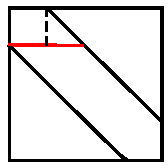
\includegraphics[scale = 0.25]{1.png}
        \end{center}
    \end{itemize}
\end{frame}

\begin{frame}{一道奇妙的题}
    \begin{itemize}
        \item 我们需要分别求出,到达每个终点的所有路径的权值之和 \pause
        \item 可以发现每一步都必然会导致所在的行$+1$,因此我们考虑按行构造生成函数 \pause
        \item 我们用$x$的指数来代表当前所在的列数,每次我们要么使得当前的列不变,要么使得当前的列$+1$ \pause
        \item 因此$F_i=dp[i][n]$的OGF为
        $$\begin{aligned}
            F(x) = x\prod_{i = 1} ^ {n - 1}(1 + (i + 1)x)
        \end{aligned}$$ 
        \item 注意第一步必定是由$(0,0)$走到$(1,1)$,因此这里要乘上$x$
    \end{itemize}
\end{frame}

\begin{frame}{一道奇妙的题}
    \begin{itemize}
        \item 很不幸,这个东西仍然不好求 \pause
        \item 再将这个多项式转化一下 \pause
        \item 由于总步数为$n$,因此如果我们知道了向下走了多少步,那么我们也就知道了向右下走了多少步 \pause
        \item 将向下走一步看作$x$,那么最终多项式中$x^i$的系数就是原多项式中$x^{n - i}$的系数 \pause
        $$\begin{aligned}
            F_1(x) = \prod_{i = 1}^{n - 1} (x + i + 1)
        \end{aligned}$$
    \end{itemize}
\end{frame}

\begin{frame}{这种奇形怪状的东西是可以求的}
    \begin{itemize}
        \item 记$G_t(x)=\prod_{i = 1} ^ {2 ^ t} (x + i + 1)$ \pause
        \item 如果我们能算出所有的$G$,那么我们就可以用类似快速幂的方法算出原多项式 \pause
        $$\begin{aligned}
            G_{t + 1}(x) = G_t(x)\times G_t(x + 2^t)
        \end{aligned}$$ \pause
        \item 记$a_i = [x^i]G_t(x),b = 2^t$ \pause
        $$\begin{aligned}
            G_{t}(x + b) = \sum_{i\geq 0}a_i\times (x + b)^i
        \end{aligned}$$ \pause
        \item 二项式定理展开
    \end{itemize}
\end{frame}

\begin{frame}{这一页是展开}
    $$\begin{aligned}
        G_t(x + b) &= \sum_{i\geq 0}a_i\times (x + b)^i\\
        &= \sum_{i\geq 0}a_i\sum_{j = 0}^i{i\choose j}x^jb^{i-j}\\
        &= \sum_{j\geq 0}x^j\sum_{i\geq j}a_ib^{i-j}\frac{i!}{j!(i-j)!}\\
        &= \sum_{j\geq 0}\frac{x^j}{j!}\sum_{i\geq j}(a_ii!)\times \frac{b^{i - j}}{(i - j)!}
    \end{aligned}$$ \pause
    \begin{itemize}
        \item 记$A(x) = \sum_{i\geq 0}a_{i}i!x^{n-i},B(x)=\sum_{i\geq 0}\frac{b^i}{i!}x^i$
        \item 第$j$项的$\sum$为$A(x)\times B(x)$的第$n-j$项的系数
    \end{itemize}
\end{frame}

\begin{frame}{又一道题}
    \begin{block}{一道不知道从哪里来的题}
        \begin{itemize}
            \item 有一个离散随机变量$x$,一开始它有$p_i$的概率是$i$
            \item 现在要对$x$进行$m$次操作,每次会将$x$等概率地变为$[0,x]$中的一个整数
            \item 问最后$x$变为$0,1,2,\cdots n$的概率
            $$\begin{aligned}
                n\leq 2.5\times 10^5,m\leq 10^{18}
            \end{aligned}$$
        \end{itemize}
    \end{block}
\end{frame}

\begin{frame}{一道不知道从哪里来的题}
    \begin{itemize}
        \item 设一开始$x$的概率生成函数为$F(x)$,经过一次操作之后的概率生成函数为$F_1(x)$ \pause
        $$\begin{aligned}
            {[x^i] }F_1(x) &= \sum_{j = i}^n \frac{[x^j]F(x)}{j + 1}\\
            F_1(x) &= \sum_{i = 0}^nx^i\sum_{j = i}^n\frac{[x^j]F(x)}{j + 1}\\
            &= \sum_{j = 0}^n\frac{[x^j]F(x)}{j + 1}\sum_{i = 0}^j x^i\\
            &= \frac{1}{x - 1}\sum_{j = 0}^n[x^j]F(x)\frac{x^{j + 1} - 1}{j + 1}
        \end{aligned}$$
    \end{itemize}
\end{frame}

\begin{frame}{一些神仙操作}
    \begin{itemize}
        \item 有一件事情 \pause
        $$\begin{aligned}
            \frac{x^{j + 1} - 1}{j + 1} = \left[\frac{t^{j + 1}}{j + 1}\right]_1^x = \int_{1}^{x}t^j  \,\mathrm{d}x 
        \end{aligned}$$ \pause
        \item 嘿嘿嘿
        $$\begin{aligned}
            F_1(x) &= \frac{1}{x - 1}\sum_{j = 0}^n[x^j]F(x)\int_{1}^{x}t^j  \,\mathrm{d}x\\
            &= \frac{1}{x - 1}\int_{1}^{x}\sum_{j = 0}^n[x^j]F(x)t^j \,\mathrm{d}x\\
            &= \frac{1}{x - 1}\int_{1}^{x}F(t)\,\mathrm{d}x
        \end{aligned}$$
    \end{itemize}
\end{frame}

\begin{frame}{转化}
    \begin{itemize}
        \item 这个东西的分母是$x - 1$,而且积分是从$1$开始积的。$x - 1$意味着这个分母不好消,从$1$开始积意味着我们需要算出$F(1)$ \pause
        \item 设$G(x) = F(x + 1), G_1(x) = F_1(x + 1)$ \pause
        $$\begin{aligned}
            G_1(x) = F_1(x + 1) = \frac{1}{x}\int_{1}^{x + 1}F(t)  \,\mathrm{d}x = \frac{1}{x}\int_{0}^{x}G(t)  \,\mathrm{d}x
        \end{aligned}$$
        \item 反正我想不到
    \end{itemize}
\end{frame}

\begin{frame}{继续推式子}
    \begin{itemize}
        \item 化简这个式子,把积分弄掉 \pause
        $$
        \begin{aligned} \frac{1}{x}\int_0^xG(t)\,\mathrm{d}t&=\frac{1}{x}\int_0^x\sum_{i=0}^ng_it^i\,\mathrm{d}t\\\ &=\frac{1}{x}\sum_{i=0}^n\int_0^xg_it^i\,\mathrm{d}t\\\ &=\frac{1}{x}\sum_{i=0}^n[\frac{g_i}{i+1}t^{i+1}]_0^x\\\ &=\frac{1}{x}\sum_{i=0}^n\frac{g_i}{i+1}x^{i+1}\\\ &=\sum_{i=0}^n\frac{g_i}{i+1}x^i \end{aligned}
        $$
    \end{itemize}
\end{frame}

\begin{frame}{式子推完了}
    \begin{itemize}
        \item 这意味着我们从$G(x)$迭代到$G_1(x)$时,第$i$项的系数会除以$i + 1$ 
        \item 迭代$m$次之后会除以$(i + 1)^m$,因此我们可以快速算出$G_m(x)$ \pause
        \item 现在唯一的问题就是怎么算出$G(x) = F(x + 1)$以及$F_m(x) = G_m(x - 1)$ \pause
        \item 二项式定理展开 \pause
    \end{itemize}
\end{frame}

\begin{frame}{又一道题}
    \begin{block}{经典问题}
        有若干种颜色不同的珠子,其中重量为$i$的珠子一共有$a_i$种,每种珠子都可以无限量使用。用珠子串成一条\textbf{重量}为$n$的项链,共有多少种方法?项链允许旋转,但不允许翻转
        $$a_i, n\leq 10^5$$
    \end{block}
\end{frame}

\begin{frame}{Polya!}
    \begin{itemize}
        \item 枚举最终项链上有多少颗珠子,假设为$k$颗 \pause
        \item 设$\{a_i\}$的OGF为$G(x)$,包含$k$颗珠子的项链的OGF为$F(x)$ \pause
        $$\begin{aligned}
            F(x) &= \frac{1}{k}\sum_{i = 1}^kG(x)^{\gcd(i, k)}[x^{\frac{n\times \gcd(i, k)}{k}}]\\
            &= \frac{1}{k}\sum_{i = 1}^kG(x^{\frac{k}{\gcd(i, k)}})^{\gcd(i, k)}[x^n]
        \end{aligned}$$
        \item 可以理解为每次在$\frac{k}{\gcd(i, k)}$个位置放珠子
    \end{itemize}
\end{frame}

\begin{frame}{Polya!}
    \begin{itemize}
        \item 记答案的OGF为$A(x)$ \pause
        $$\begin{aligned}
            A(x)&=\sum_{k\geq 1}\frac{1}{k}\sum_{i=1}^kG(x^{\frac{k}{\gcd(i,k)}})^{\gcd(i,k)}\\ \pause
                &=\sum_{k\geq 1}\frac{1}{k}\sum_{i|k}\varphi(i)G(x^i)^\frac{k}{i}\\ \pause
                &=\sum_{i\geq 1}\varphi(i)\sum_{j\geq 1}\frac{G(x^i)^j}{ij}\\ \pause
                &=-\sum_{i\geq 1}\frac{\varphi(i)}{i}\ln(1-G(x^i)) \pause
        \end{aligned}$$
        \item 只要算出了$\ln(1 - G(x))$,我们也就知道了$\ln(1 - G(x^i))$
    \end{itemize}
\end{frame}

\begin{frame}{原题放送}
    \begin{block}{UOJ424 count}
        \begin{itemize}
            \item 如果一个序列满足序列长度为$n$,序列中的每个数都是$1$到$m$内的整数,且所有$1$到$m$内的整数都在序列中出现过,则称这是一个挺好序列。
            \item 对于一个序列$A$,记$f_A(l,r)$为$A$的第$l$个到第$r$​个数中最大值的下标(如果有多个最大值,取下标最小的)。
            \item 两个序列$A$和$B$同构,当且仅当$A$和$B$长度相等,且对于任意$i\leq j$,均有$f_A(i,j)=f_B(i,j)$。
            \item 给出$n,m$,求有多少种不同构的挺好序列。
            $$n, m\leq 10^5$$
        \end{itemize}
    \end{block}
\end{frame}

\begin{frame}{UOJ424 count}
    \begin{itemize}
        \item 如果不考虑$1$到$m$均出现过这一条限制,那么两个序列不同构当且仅当它们的笛卡尔树不同 \pause
        \item 注意这里我们认为一个点的左儿子的权值小于这个点的权值,其右儿子的权值小于等于这个点的权值 \pause
        \item 显然根到每个叶子往左走的次数不能超过$m-1$ \pause
        \item 事实上,当$m\leq n$时,我们并不需要保证$1$到$m$均出现过,因为此时满足最大值小于等于$m$的笛卡尔树一定能够通过调节节点的权值使得$1$到$m$均出现过 \pause
        \item 也就是说,我们实际上要统计$n$个节点,根到每个节点的路径中往左走的次数不能超过$m-1$的二叉树的数量
    \end{itemize}
\end{frame}

\begin{frame}{UOJ424 count}
    \begin{itemize}
        \item 设$f[i][j]$表示$j$个点,往左走的次数小于$i$的二叉树的数量,初值为$f[0][0] = 1$。这个东西写成生成函数就是 
        $$\begin{aligned}
            F_0(x) = 1, F_i(x) &= xF_{i - 1}(x)F_i(x) + 1\\
            &= \frac{1}{1 - xF_{i - 1}(x)}
        \end{aligned}$$ \pause
        \item 接着是非常神奇的一步,观察这个递推式,可以发现$F_t(x)$一定可以被表示成$\frac{A}{B}$的形式,这里$A,B$是两个多项式。对于$F_0(x)$来说,$A=B=1$
    \end{itemize}
\end{frame}

\begin{frame}{UOJ424 count}
    $$\begin{aligned}
        \frac{A'}{B'} &= \frac{1}{1 - x\frac{A}{B}}\\
        &= \frac{B}{B-xA} \Rightarrow A' = B, B' = B - xA
    \end{aligned}$$ \pause
    \begin{itemize}
        \item 模拟FFT的过程,代入$2^l$个点值,可以通过矩乘快速算出迭代$m$次之后的点值是啥,最后再做一次IDFT即可
    \end{itemize}
\end{frame}

\section{组合计数}

\begin{frame}{组合恒等式}
    $$\begin{aligned}
        {n\choose m} &= {n\choose n - m}\\ \pause
        \sum_{i = 0}^n {n\choose i} &= 2^n\\ \pause
        \sum_{i = 0}^n {n\choose i}[2 \mid i] &= \sum_{i = 0}^n {n\choose i}[2 \nmid i] = 2^{n - 1}\\ \pause
        \sum_{i = 0}^m {n + i\choose n} &= {n + m + 1\choose m}\\ \pause
        {n\choose m}{m\choose k} &= {n\choose k}{n - k\choose m - k}\\ \pause
        \sum_{i = 0}^k {n\choose i}{m\choose k - i} &= {n + m\choose k}
    \end{aligned}$$
\end{frame}

\begin{frame}{比较常用的转化}
    \begin{itemize}
        \item 1.将$n$个元素分为若干个集合,每种方案的权值为每个集合的大小的积
        \item 相当于先分为若干个集合,再从每个集合中选一个数 \pause
        \item 2.$X_1+X_2+\cdots + X_n = S$,对于每个$X_i$有$X_i\geq 1$,计算每种方案的$\prod X_i$之和
        \item 根据$1$,相当于将$S$分为$n$个集合后,从每个集合内再选一个数的方案数 \pause
        \item 将每个变量拆成两个变量,分别代表这个集合所选数之前有多少个数,之后有多少个数
        \item $(X_1 + Y_1) + (X_2 + Y_2) + \cdots + (X_n + Y_n) = S - n$,每个变量$\geq 1$
    \end{itemize}
\end{frame}

\begin{frame}{新鲜出炉的例题}
    \begin{block}{dict}
        \begin{itemize}
            \item 给定一个$1\cdots n$的排列$p_{1,2\cdots n}$,定义两个大小为$n$的不可重集合$A,B$的字典序比较方式为:
            \item 先比较$A$和$B$的第$p_1$消的元素,较小的那个字典序较小,否则比较第$p_2$小的元素,以此类推
            \item 现在给定$p_{1,2\cdots n}$和一个大小为$n$的不可重集合$B$,求有几个值在$1\cdots m$,大小为$n$的不可重集合$A$满足$A$的字典序比$B$小
            $$n\leq m\leq 2\times 10^5$$
        \end{itemize}
    \end{block}
\end{frame}

\begin{frame}{dict}
    \begin{itemize}
        \item 由于是比较字典序的大小,因此我们可以枚举它们的lcp,即在哪一次比较中,$A$的元素比$B$的对应元素小 \pause
        \item 在这一位之前,$A$必须与$B$相同,在这一位之后,$A$可以随便填 \pause
        \item 假设此时比较到了第$i$位,这就意味着$p_1,p_2,\cdots p_{i - 1}$这些位置中的数已经确定了 \pause
        \item 假设在这些位置之中,比$p_i$小的最大的位置为$p_j$,比$p_i$大的最小的位置为$p_k$ \pause
        \item 显然$p_i$这个位置无论怎么填都不会影响到$p_j$之前、$p_k$之后的位置,这些位置的方案数是确定的
    \end{itemize}
\end{frame}

\begin{frame}{dict}
    \begin{itemize}
        \item 枚举$A_{p_i} - A_{p_j}$,可以发现我们实际上要求的是一个类似这样的式子 \pause
        $$\begin{aligned}
            \sum_{i = 1}^r {i - 1\choose a} \times {t - i\choose b}
        \end{aligned}$$ \pause
        \item 当$a$能取到$t$的上界时,这就是一个简单的组合恒等式,它等于${t\choose a + b + 1}$ \pause
        \item 如果$t - a$比较小,我们可以暴力枚举$i$,否则用总数减去不合法的情况 \pause
        \item 这实际上是一个启发式分裂的过程,因此时间复杂度为$O(n\log n)$
    \end{itemize}
\end{frame}

\begin{frame}{它lei了}
    \begin{block}{青春猪头少年不会梦到兔女郎学姐}
        \begin{itemize}
            \item 有$n$种球,第$i$种球有$a_i$个
            \item 对于一个序列,将其看作是首位相连的。一个序列的权值为每个极大相同颜色段的长度的乘积,求所有序列的权值之和
            \item $\sum a_i\leq 2\times 10^5$
        \end{itemize}
    \end{block}
\end{frame}

\begin{frame}{青春猪头少年不会梦到兔女郎学姐}
    \begin{itemize}
        \item 我们先考虑这样一个问题:有$n$种球,第$i$种球有$a_i$个,规定相邻两个位置的球不能相同,问方案数 \pause
        \item 考虑第$i$种球,假设它们出现了$j$对相邻的情况,那么我们可以将这些相邻的球缩在一起。即从原来的$i$个球缩为了$i - j$个球,同时乘上容斥系数$(-1)^j{i - 1\choose j}$,最后再将剩下的球可重排列一下 \pause
        \item 回到这道题,如果我们确定了每种颜色最后的分段情况是啥样的,那么就转化为了上面那个问题 \pause
        \item 来点式子
    \end{itemize}
\end{frame}

\begin{frame}{青春猪头少年不会梦到兔女郎学姐}
    \begin{itemize}
        \item 我们先只考虑链的情况,定义$f(a, b)$表示将$a$个球分为$b$段,所有方案的权值之和 \pause
        \item 那么一种球的EGF为
        $$\begin{aligned}
            \hat A_i(x) &= \sum_{j = 1}^{a_i} f(a_i, j) \sum_{k = 1} ^ j{j - 1\choose j - k}(-1)^{j - k}\frac{x^k}{k!}\\
            &= \sum_{k = 1}^{a_i}\frac{x^k}{k!}(-1)^k \sum_{j = k}^{a_i} f(a_i, j)(-1)^j{j - 1\choose j - k}
        \end{aligned}$$
    \end{itemize}
\end{frame}

\begin{frame}{青春猪头少年不会梦到兔女郎学姐}
    \begin{itemize}
        \item 有一个问题:$f(a, b)$咋求 \pause
        \item 用之前提到的方法,可以发现$f(a, b) = {a - b - 1\choose 2b - 1}$,因此 \pause
        $$\begin{aligned}
            \hat A_i(x) &= \sum_{k = 1}^{a_i}\frac{x^k}{k!}(-1)^k \sum_{j = k}^{a_i} f(a_i, j)(-1)^j{j - 1\choose j - k}\\ \pause
            &= \sum_{k = 1}^{a_i}\frac{x^k}{k!}(-1)^k \sum_{j = k}^{a_i}{a_i - j - 1\choose 2j - 1}(-1^j)\frac{(j - 1)!}{(j - k)!(k - 1)!}\\ \pause
            &= \sum_{k = 1}^{a_i}\frac{x^k}{k!(k - 1)!}(-1)^k \sum_{j = k}^{a_i}{a_i - j - 1\choose 2j - 1}(-1)^j(j - 1)!\times \frac{1}{(j - k)}\\ \pause
        \end{aligned}$$
        \item 由于$\sum a_i = O(n)$,因此算出所有$\hat A_i(x)$的复杂度为$O(n\log n)$
    \end{itemize}
\end{frame}

\begin{frame}{青春猪头少年不会梦到兔女郎学姐}
    \begin{itemize}
        \item 有环怎么办?\pause
        \item 我们钦定环的开头为第一种球,并且结尾不是第一种球,此时可以将环断为链,答案不变 \pause
        \item 此时每一种方案都可以转$m = \sum a_i$次,如果一种方案中第一种球被分为了$k$段,那么这种方案被计算了$k$次 \pause
        \item 我们将第一种球的EGF单独拿出来,如果我们钦定开头为第一种球,那么这个EGF里面的$\frac{x^i}{i!}$应该变为$\frac{x^{i - 1}}{(i - 1)!}$ \pause
        \item 如果我们钦定开头结尾都是第一种球,那么$\frac{x^i}{i!}$应该变为$\frac{x^{i - 2}}{(i - 2)!}$ \pause
        \item 注意要去掉多算的情况,因此要将含$j$的项除以$j$
    \end{itemize}
\end{frame}

\section{斯特林反演}

\begin{frame}{关于斯特林数}
    \begin{itemize}
        \item 第一类斯特林数:将$n$个元素划分为$m$个圆排列的方案数 \pause
        \item 第二类斯特林数:将$n$个元素花费为$m$个集合的方案数 \pause
        $$\begin{aligned}
            \begin{bmatrix}n\\m\end{bmatrix} &= \begin{bmatrix}n - 1\\m - 1\end{bmatrix} + (n - 1)\begin{bmatrix}n - 1\\m\end{bmatrix}\\
            \begin{Bmatrix}n\\m\end{Bmatrix} &= \begin{Bmatrix}n - 1\\m - 1\end{Bmatrix} + m\begin{Bmatrix}n - 1\\m\end{Bmatrix}\\
            \begin{Bmatrix}n\\m\end{Bmatrix} &= \frac{1}{m!}\sum_{k = 0}^m(-1)^k {m\choose k}(m - k)^n
        \end{aligned}$$
    \end{itemize}
\end{frame}

\begin{frame}{一些引理以及推论}
    $$\begin{gathered}
        n^m = \sum_{i = 0}^m \begin{Bmatrix}m\\ i\end{Bmatrix}n^{\underline{i}}\\
        n^{\overline{m}} = \sum_{i = 0}^m \begin{bmatrix}m\\ i\end{bmatrix}n^i\\
        [n = m] = \sum_{k = m}^n(-1)^{n - k}\begin{bmatrix}n\\ k\end{bmatrix}\begin{Bmatrix}k\\ m\end{Bmatrix}\\
        [n = m] = \sum_{k = m}^n(-1)^{n - k}\begin{Bmatrix}n\\ k\end{Bmatrix}\begin{bmatrix}k\\ m\end{bmatrix}\\
        x^{\underline{n}} = (-1)^n (-x)^{\overline{n}} , x^{\overline{n}} = (-1)^n (-x)^{\underline{n}}
    \end{gathered}$$
\end{frame}

\begin{frame}{证明}
    $$n^m = \sum_{i = 0}^m \begin{Bmatrix}m\\ i\end{Bmatrix}n^{\underline{i}}$$ \pause
    \begin{itemize}
        \item 考虑$n^m$的组合意义,即有序地选$m$个$1\sim n$的数,可以相同的方案数 \pause
        \item 枚举这$m$个数中有多少种不同的数,然后将相同的数缩在一起。此时一共有$i$个数,限制变为每个数都不能相同,因此一共有$n^{\underline{i}}$种方案 \pause
        \item 这个式子也可以写成
        $$n^m = \sum_{i = 0}^m \begin{Bmatrix}m\\ i\end{Bmatrix}i!{n\choose i}$$
    \end{itemize}
\end{frame}

\begin{frame}{证明}
    $$\begin{aligned}
        n^{\underline{m}} &= \sum_{i = 0}^m \begin{bmatrix}m\\ i\end{bmatrix}n^i(-1)^{i - m}\\
        n^{\overline{m}} &= \sum_{i = 0}^m \begin{bmatrix}m\\ i\end{bmatrix}n^i
    \end{aligned}$$ \pause
    \begin{itemize}
        \item 采用数学归纳法证明
        \item 这一页写不下了
    \end{itemize}
\end{frame}

\begin{frame}{证明}
    $$\begin{aligned}
        n^{\overline{m}} &= (n + m - 1)n^{\overline{m - 1}}\\
        &= (n + m - 1)\sum_{i = 0}^{m - 1}\begin{bmatrix}m - 1\\ i\end{bmatrix}n^i\\
        &= \sum_{i = 0}^{m - 1}\begin{bmatrix}m - 1\\ i\end{bmatrix}n^{i + 1} + \sum_{i = 0}^{m - 1}\begin{bmatrix}m - 1\\ i\end{bmatrix}n^i(m - 1)\\
        &= \sum_{i = 1}^{m}\begin{bmatrix}m - 1\\ i - 1\end{bmatrix}n^{i} + \sum_{i = 0}^{m - 1}\begin{bmatrix}m - 1\\ i\end{bmatrix}n^i(m - 1)\\
        &= \sum_{i = 0}^m\left(\begin{bmatrix}m - 1\\ i - 1\end{bmatrix} + (m - 1)\begin{bmatrix}m - 1\\ i\end{bmatrix}\right)n^i\\
        &= \sum_{i = 0}^m \begin{bmatrix}m\\ i\end{bmatrix}n^i
    \end{aligned}$$
\end{frame}

\begin{frame}{反转公式}
    $$\begin{aligned}
        \ [n = m] &= \sum_{k = m}^n(-1)^{n - k}\begin{bmatrix}n\\ k\end{bmatrix}\begin{Bmatrix}k\\ m\end{Bmatrix}\\
        [n = m] &= \sum_{k = m}^n(-1)^{n - k}\begin{Bmatrix}n\\ k\end{Bmatrix}\begin{bmatrix}k\\ m\end{bmatrix}
    \end{aligned}$$ \pause
    \begin{itemize}
        \item 第二个的证明是结合正常幂转下降幂、上升幂转正常幂
        \item 第一个的证明可以结合下降幂转正常幂、正常幂转下降幂 \pause
        \item 不出意外的话,这一页又写不下了
    \end{itemize}
\end{frame}

\begin{frame}{证明}
    $$\begin{aligned}
        n^m &= \sum_{i = 0}^m\begin{Bmatrix}m\\ i\end{Bmatrix}n^{\underline{i}}\\ \pause
            &= \sum_{i = 0}^m\begin{Bmatrix}m\\ i\end{Bmatrix}(-1)^i(-n)^{\overline{i}}\\ \pause
            &= \sum_{i = 0}^m\begin{Bmatrix}m\\ i\end{Bmatrix}(-1)^i\sum_{j = 0}^i\begin{bmatrix}i\\ j\end{bmatrix}(-n)^j\\ \pause
            &= \sum_{j = 0}^mn^j\sum_{i = j}^m\begin{Bmatrix}m\\ i\end{Bmatrix}\begin{bmatrix}i\\ j\end{bmatrix}(-1)^{i-j} \pause
    \end{aligned}$$
    \begin{itemize}
        \item 第二个$\sum$里面的项是与$n$无关的,但是$n$无论为何值的时候这个等式都成立,因此反转公式成立
    \end{itemize}
\end{frame}

\begin{frame}{斯特林反演}
    $$\begin{gathered}
        f(n) = \sum_{k = 0}^n\begin{Bmatrix}n\\ k\end{Bmatrix}g(k)\Leftrightarrow g(n) = \sum_{k = 0}^n(-1)^{n - k}\begin{bmatrix}n\\ k\end{bmatrix}f(k)\\
        f(n) = \sum_{k = 0}^n\begin{bmatrix}n\\ k\end{bmatrix}g(k)\Leftrightarrow g(n) = \sum_{k = 0}^n(-1)^{n - k}\begin{Bmatrix}n\\ k\end{Bmatrix}f(k)\\
        f(n) = \sum_{k\geq n}\begin{Bmatrix}k\\ n\end{Bmatrix}g(k)\Leftrightarrow g(n) = \sum_{k\geq n}(-1)^{k - n}\begin{bmatrix}k\\ n\end{bmatrix}f(k)
    \end{gathered}$$ \pause
    \begin{itemize}
        \item 我们接下来证明第一个,第二个的证明与之类似 \pause
        \item 假设有
        $$g(n) = \sum_{k = 0}^n(-1)^{n - k}\begin{bmatrix}n\\ k\end{bmatrix}f(k)$$
    \end{itemize}
\end{frame}

\begin{frame}{斯特林反演}
    $$\begin{aligned}
        f(n) &= \sum_{i = 0}^n [i = n]f(i)\\ \pause
        &= \sum_{i = 0}^n\sum_{j = i}^n\begin{Bmatrix}n\\ j\end{Bmatrix}\begin{bmatrix}j\\ i\end{bmatrix}(-1)^{j - i}f(i)\\ \pause
        &= \sum_{j = 0}^n\begin{Bmatrix}n\\ j\end{Bmatrix}\sum_{i = 0}^j\begin{bmatrix}j\\ i\end{bmatrix}(-1)^{j - i}f(i)\\ \pause
        &= \sum_{j = 0}^n\begin{Bmatrix}n\\ j\end{Bmatrix}g(j)
    \end{aligned}$$
\end{frame}

\begin{frame}{再放送}
    \begin{block}{CF1278F Cards}
        \begin{itemize}
            \item 有$m$张牌,其中有一张是王牌,现在进行$n$次洗牌,每次洗牌之后查看第一张牌是什么
            \item 令$x$为洗牌后第一张牌为王牌的次数,求$x^k$的期望
            $$n,m\leq 998244353,k\leq 5000$$
        \end{itemize}
    \end{block}
    \begin{itemize}
        \item 建议试试运用之前的公式爆推式子
    \end{itemize}
\end{frame}

\begin{frame}{CF1278F Cards}
    $$\begin{aligned}
        ans &= \frac{1}{m^n}\sum_{i = 1}^n{n\choose i}(m - 1)^{n - i}i^k\\ \pause
        &= \frac{1}{m^n}\sum_{i = 1}^n{n\choose i}(m - 1)^{n - i}\sum_{j = 0}^k\begin{Bmatrix}k\\ j\end{Bmatrix}{i\choose j}j!\\ \pause
        &= \frac{1}{m^n}\sum_{j = 0}^k\begin{Bmatrix}k\\ j\end{Bmatrix}j!\sum_{i = 1}^n{n\choose i}{i\choose j}(m - 1)^{n - i}\\ \pause
        &= \frac{1}{m^n}\sum_{j = 0}^k\begin{Bmatrix}k\\ j\end{Bmatrix}j!{n\choose j}\sum_{i = 1}^n{n - j\choose i - j}(m - 1)^{n - i}\\ \pause
        &= \frac{1}{m^n}\sum_{j = 0}^k\begin{Bmatrix}k\\ j\end{Bmatrix}j!{n\choose j}m^{n - j}
    \end{aligned}$$
\end{frame}

\begin{frame}{一道例题}
    \begin{block}{异或图}
        给定$S$个点集大小为$N$的图,问有多少个图的集合异或结果为一个连通图
        $$N\leq 10, S\leq 60$$
    \end{block}
\end{frame}

\begin{frame}{异或图}
    \begin{itemize}
        \item 设$g(n)$表示将所有点恰好分为$n$个连通块的方案数 \pause
        \item $f(n)$表示将所有点划分为$n$个集合,不同集合直接一定不连通,集合内部可以连通,也可以不连通的方案数 \pause
        \item 枚举$n$的集合划分,问题转化为有若干个异或方程,求解的个数,可以上线性基 \pause
        $$\begin{aligned}
            f(n) &= \sum_{i\geq n} \begin{Bmatrix}i\\ n\end{Bmatrix}g(i)\\
            g(n) &= \sum_{i\geq n} \begin{bmatrix}i\\ n\end{bmatrix}f(i)(-1)^{i - n}\\
            g(1) &= \sum_{i\geq 1} (-1)^{i - 1}(n - 1)!f(i)
        \end{aligned}$$
    \end{itemize}
\end{frame}

\begin{frame}{另一道题}
    \begin{block}{戴老师ppt里的}
        求$n$个点的带标号无向图的连通块数的$k$次方幂之和
        $$n\leq 10^5, k\leq 15$$
    \end{block}
\end{frame}

\begin{frame}{另一道题}
    \begin{itemize}
        \item $n$个点带标号连通图的数量很好求,我们记它的EGF为$\hat G(x)$ \pause
        \item 设$n$个点带标号无向图的EGF为$\hat F(x)$ \pause
        $$\begin{aligned}
            \hat F(x) &= \sum_{i\geq 0}\frac{\hat G(x)^i}{i!}\\
            &= \exp \hat G(x)\\
            \hat G(x) &= \ln \hat F(x)
        \end{aligned}$$
    \end{itemize}
\end{frame}

\begin{frame}{另一道题}
    \begin{itemize}
        \item 先将$k$次方幂拆开
        $$m^k=\sum_{i = 0}^k\begin{Bmatrix}k\\ i\end{Bmatrix}{m\choose i}i!$$ \pause
        \item 也就是说,如果一张图有$m$个连通块,我们需要计算出从这$m$个连通块中选出$i$个连通块的方案数之和 \pause
        \item 记$\hat H_k(x)$为无向图从所有连通块中选出$k$个连通块的方案数
    \end{itemize}
\end{frame}

\begin{frame}{另一道题}
    $$\begin{aligned}
        \hat H_k(x) &= \sum_{i\geq 0}\frac{\hat G(x)^i}{i!}{i\choose k}\\
        &= \sum_{i\geq 0}\frac{\hat G(x)^i}{i!}\times \frac{i!}{k!(i - k)!}\\
        &= \frac{1}{k!}\sum_{i\geq 0}\frac{\hat G(x)^i}{(i - k)!}\\
        &= \frac{\hat G(x)^k}{k!}\sum_{i\geq 0}\frac{\hat G(x)^{i - k}}{(i - k)!}\\
        &= \frac{\hat G(x)^k}{k!}\exp \hat G(x) = \frac{\hat G(x)^k}{k!}F(x)
    \end{aligned}$$
\end{frame}

\begin{frame}{它lei了}
    \begin{block}{清华集训2017 生成树计数}
        \begin{itemize}
            \item 在一个$s$个点的图中,存在$s - n$条边,使图中形成了$n$个连通块,第$i$个连通块中有$a_i$个点
            \item 现在我们需要再连接$n - 1$条边,使该图变成一棵树。对于一种连边方案,设原图中第$i$个连通块连出了$d_i$条边,那么这棵树$T$的价值为
            $$\mathrm{val}(x) = \left(\prod_{i = 1}^n d_i^m\right)\left(\sum_{i = n}^nd_i^m\right)$$
            \item 求所有可能的生成树的价值之和
            $$n\leq 3\times 10^4, m\leq 30$$
            \item 在座的各位有谁能现场想出来我当场把zzh吃掉
        \end{itemize}
    \end{block}
\end{frame}

\begin{frame}{清华集训2017 生成树计数}
    \begin{itemize}
        \item 将一开始就连通的点缩起来,我们考虑枚举缩点之后的一棵生成树$T$ \pause
        $$ans = \sum_{T}\sum_{i = 1}^n d_i^m \prod_{j = 1}^nd_j^m a_j^{d_j}$$ \pause
        \item 需要注意的是缩点之后每个连通块连出的边都可以选择这个连通块内的任意一个点作为起点,因此每条边都有$a_j$种选法。一个连通块连出了$d_j$条边,总方案数为$a_j^{d_j}$ \pause
        \item 将$\prod$中$i = j$的项提到前面来
        $$ans = \sum_{T}\sum_{i = 1}^n d_i^{2m} a_i^{d_i} \prod_{j\neq i} d_j^m a_j^{d_j}$$
    \end{itemize}
\end{frame}

\begin{frame}{清华集训2017 生成树计数}
    \begin{itemize}
        \item 枚举生成树的一种方法就是使用prufer序,考虑枚举每个点在prufer序中的出现次数$c_i$,那么有$d_i = c_i + 1$ \pause
        \item 对于一个长度为$n - 2$的prufer序,如果我们知道了每个点的出现次数,那么对应的序列就有$\frac{(n - 2)!}{\prod c_i!}$种 \pause
        $$ans = \sum_{\sum c_i = n - 2} \frac{(n - 2)!}{\prod c_i!} \sum_{i = 1}^n (c_i + 1)^{2m} a_i^{c_i + 1} \prod_{j\neq i} (c_j + 1)^m a_j^{c_j + 1}$$
    \end{itemize}
\end{frame}

\begin{frame}{清华集训2017 生成树计数}
    \begin{itemize}
        \item 考虑根据这个式子构造EGF \pause
        \item 由于我们要满足$\sum c_i = n - 2$,不妨将$c_i$作为指数 \pause
        $$\begin{aligned}
            \hat A_i(x) &= \sum_{k} a_i^{k + 1} (k + 1)^{2m} \frac{x^k}{k!}\\
            \hat B_i(x) &= \sum_{k} a_i^{k + 1} (k + 1)^m \frac{x^k}{k!}
        \end{aligned}$$ \pause
        \item 单独考虑每个点对答案的贡献,可以得到
        $$ans = (n - 2)![x^{n - 2}]\sum_{i - 1}^n A_i(x)\prod_{j\neq i}B_j(x)$$
    \end{itemize}
\end{frame}

\begin{frame}{清华集训2017 生成树计数}
    \begin{itemize}
        \item 化简$A_i(x), B_i(x)$:先积分,再求导 \pause
        $$\begin{aligned}
            T_i(x) &= \int \hat A_i(x)\,\mathrm{d}x = \sum_{k} a_i^{k + 1} \frac{(k + 1)^{2m}}{(k + 1)!} x^{k + 1}\\ \pause
            &= \sum_{k} a_i^k \frac{k^{2m}}{k!} x^k = \sum_{k} a_i^k \sum_{j = 0}^{2m} \begin{Bmatrix}2m\\ j\end{Bmatrix}\frac{k!}{(k - j)!}\times \frac{1}{k!} x^k\\ \pause
            &= \sum_{j = 0}^{2m} \begin{Bmatrix}2m\\ j\end{Bmatrix} a_i^j x^j \sum_{k} \frac{(a_ix)^{k - j}}{(k - j)!}\\ \pause
            &= \sum_{j = 0}^{2m} \begin{Bmatrix}2m\\ j\end{Bmatrix} a_i^j x^j \exp a_ix 
        \end{aligned}$$
    \end{itemize}
\end{frame}

\begin{frame}{清华集训2017 生成树计数}
    \begin{itemize}
        \item 然后我们再求导回去 \pause
        $$\begin{aligned}
            A_i(x) &= T_i'(x) = \left[e^{a_ix}\left(\sum_{j = 0}^{2m} \begin{Bmatrix}2m\\ j\end{Bmatrix} a_i^j x^j \right) \right]'\\ \pause
            &= e^{a_ix}\sum_{j = 0}^{2m} \begin{Bmatrix}2m\\ j + 1\end{Bmatrix} a_i^{j + 1} (j + 1) x^j + a_i \sum_{j = 0}^{2m} \begin{Bmatrix}2m\\ j\end{Bmatrix} a_i^j x^j e^{a_ix}\\ \pause
            &= e^{a_ix}\sum_{j = 0}^{2m} a_i^{j + 1}x^j \left(\begin{Bmatrix}2m\\ j + 1\end{Bmatrix}(j + 1) + \begin{Bmatrix}2m\\ j\end{Bmatrix}\right)\\ \pause
            &= e^{a_ix}\sum_{j = 0}^{2m} a_i^{j + 1}x^j \begin{Bmatrix}2m + 1\\ j + 1\end{Bmatrix}
        \end{aligned}$$
    \end{itemize}
\end{frame}

\begin{frame}{清华集训2017 生成树计数}
    \begin{itemize}
        \item 同理,我们可以得出
        $$\begin{aligned}
            B_i(x) = e^{a_ix}\sum_{j = 0}^{m} a_i^{j + 1}x^j \begin{Bmatrix}m + 1\\ j + 1\end{Bmatrix}
        \end{aligned}$$ \pause
        \item 记$A_i(x) = e^{a_ix}A^1_i(x), B_i(x) = e^{a_ix}B^1_i(x)$ \pause
        $$\begin{aligned}
            ans &= (n - 2)![x^{n - 2}]\sum_{i - 1}^n A_i(x)\prod_{j\neq i}B_j(x)\\ \pause
            &= (n - 2)![x^{n - 2}]e^{\sum a_ix} \sum_{i = 1}^n A^1_i(x) \prod_{j\neq i} B^1_j(x)
        \end{aligned}$$
    \end{itemize}
\end{frame}

\begin{frame}{清华集训2017 生成树计数}
    \begin{itemize}
        \item 每个$A^1_i(x)$都只有$2m$项,每个$B^1_i(x)$都只有$m$项 \pause
        \item 等式右边的那个东西可以用分治NTT求出来,维护区间的答案以及区间$B^1_i(x)$的乘积即可 \pause
        \item 将$e^{\sum a_ix}$展开,注意我们只需要计算$x^{n - 2}$的系数 \pause
        \item 时间复杂度$O(nm\log n)$
    \end{itemize}
\end{frame}

\begin{frame}{But}
    \begin{itemize}
        \item 你会在洛谷T飞 \pause
        \item 需要用到一些神仙优化
    \end{itemize}
\end{frame}

\begin{frame}{清华集训2017 生成树计数}
    \begin{itemize}
        \item 令
        $$\begin{aligned}
            A(x) &= \sum_{k} \frac{(k + 1)^{2m}}{k!} x^k\\
            B(x) &= \sum_{k} \frac{(k + 1)^{m}}{k!} x^k \pause
        \end{aligned}$$
        \item 对比之前的式子,可以得到
        $$\begin{aligned}
            ans = (n - 2)!\prod a_i [x^{n - 2}] \sum_{i = 1}^n A(a_ix) \prod_{j\neq i} B(a_jx)
        \end{aligned}$$
    \end{itemize}
\end{frame}

\begin{frame}{清华集训2017 生成树计数}
    $$\begin{aligned}
        F(x) &= \sum_{i = 1}^n A(a_ix) \prod_{j\neq i} B(a_jx)\\
        &= \prod_{j = 1}^n B(a_jx) \sum_{i = 1}^n \frac{A(a_ix)}{B(a_ix)}\\
        &= \exp \left(\sum_{j = 1}^n \ln B(a_jx)\right) \sum_{i = 1}^n \frac{A(a_ix)}{B(a_ix)} \pause
    \end{aligned}$$
    \begin{itemize}
        \item 如果我们求出了$\ln B(x), \frac{A(x)}{B(x)}$,那么只需要将$\sum a_i^k$乘到这两个多项式$x^k$的系数上,就可以得出$\sum \ln B(a_jx)$和$\sum \frac{A(a_ix)}{B(a_ix)}$
    \end{itemize}
\end{frame}

\begin{frame}{清华集训2017 生成树计数}
    \begin{itemize}
        \item 对于任意的$k\in [1, n]$,求出$\sum a_i^k$ \pause
        $$\begin{aligned}
            G(x) &= \sum_{k\geq 0} \sum_{i = 1}^n a_i^kx^k\\
            &= \sum_{i = 1}^n \sum_{k\geq 0} (a_ix)^k = \sum_{i = 1}^n \frac{1}{1 - a_ix}\\ \pause
            &= \sum_{i = 1}^n \left(1 + \frac{a_ix}{1 - a_ix}\right) = n - x\sum_{i = 1}^n (\ln 1 - a_ix)'\\ \pause
            &= n - x\left[\ln \prod_{i = 1}^n (1 - a_ix)\right]'
        \end{aligned}$$
    \end{itemize}
\end{frame}

\section{单位根反演}

\begin{frame}{单位根反演是啥}
    \begin{itemize}
        \item 我们称主$n$次单位根$\omega_n = \cos \frac{2\pi}{n} + \sin \frac{2\pi}{n}i$。在FFT的过程中带入的实际上就是$\omega_n^0$到$\omega_n^{n - 1}$ \pause
        \item 如果有模数$p$,那么我们可以求出$p$的原根$g$,在模$p$意义下的主$n$次单位根就是$g^{\frac{p - 1}{n}}$ \pause
        \item 单位根反演:
        $$\begin{aligned}
            \ [n\mid k] = \frac{1}{n} \sum_{i = 0}^{n - 1} (\omega_n^k)^i
        \end{aligned}$$
    \end{itemize}
\end{frame}

\begin{frame}{单位根反演是啥}
    \begin{itemize}
        \item 当$n\mid k$时,$\omega_n^k = 1$,等式显然成立 \pause
        \item 否则,等式右边是一个等比数列,且公比不为$1$ \pause
        $$\begin{aligned}
            \sum_{i = 0}^{n - 1} (\omega_n^k)^i = \frac{\omega_n^{kn} - 1}{\omega_n^k - 1} = 0
        \end{aligned}$$
    \end{itemize}
\end{frame}

\begin{frame}{关于Bluestein}
    \begin{itemize}
        \item 任意长度DFT \pause
        \item 在DFT的过程中,我们想要求出原多项式在$\omega_{n}^k$处的点值
        $$\begin{aligned}
            y_k = \sum_{i = 0}^{n - 1}a_i\omega_n^{ki} \pause
        \end{aligned}$$ 
        \item $ki$没法用卷积表示,可以考虑将其拆成$\frac{k^2 + i^2 - (k - i)^2}{2}$ \pause
        $$\begin{aligned}
            y_k &= \sum_{i = 0}^{n - 1}a_i\omega_{2n}^{k^2 + i^2 - (k - i)^2}\\ \pause
            &= \omega_{2n}^{k^2}\sum_{i = 0}^{n - 1}a_i\omega_{2n}^{i^2}\times \omega_{2n}^{-(k - i)^2}
        \end{aligned}$$
    \end{itemize}
\end{frame}

\begin{frame}{一道例题}
    \begin{block}{白兔之舞}
        \begin{itemize}
            \item 有一张$n$行$L + 1$列的有向图,$(x_1, y_1)$到$(x_2, y_2)$之间有$w[x_1][x_2]$条边$(x_1 < x_2)$
            \item 对于$i\in [0, k)$,求出有多少条从$(x, 0)$出发,终止节点所在的行为$y$,且长度模$k$为$i$的路径
            \item 答案对质数$p$取模
            $$n\leq 3, L\leq 10^8, 10^8 < p < 2^{32}, k \mid p - 1, k < 65536$$
        \end{itemize}
    \end{block}
\end{frame}

\begin{frame}{白兔之舞}
    \begin{itemize}
        \item 考虑$n = 1$怎么做 \pause
        \item 令$v = w[1][1]$,那么我们实际上要求的是 
        $$\begin{aligned}
            y_t = \sum_{i = 0}^L v^i {L\choose i} [k\mid i - t] \pause
        \end{aligned}$$
        \item 代入反演公式
        $$\begin{aligned}
            y_t &= \sum_{i = 0}^L v^i {L\choose i} \frac{1}{k} \sum_{j = 0}^{k - 1} (\omega_k^{i - t})^j\\
            &= \frac{1}{k}\sum_{j = 0}^{k - 1} \omega_{k}^{-tj} \sum_{i = 0}^L v^i {L\choose i} \omega_{k}^{ij}
        \end{aligned}$$
    \end{itemize}
\end{frame}

\begin{frame}{白兔之舞}
    \begin{itemize}
        \item 最右边是一个长的很像二项式定理的东西 \pause
        $$\begin{aligned}
            y_t &= \frac{1}{k}\sum_{j = 0}^{k - 1} \omega_{k}^{-tj} (1 + v\omega_{k}^j)^L \pause
        \end{aligned}$$
        \item 又出现了熟悉的$-tj$,但是这次我们不能将其拆成$\frac{t^2 + j^2 - (t + j)^2}{2}$,因为$\omega_{2k}$在模$p$意义下不一定存在 \pause
        \item 拆成${t\choose 2} + {j\choose 2} - {t + j\choose 2}$可以完美解决问题 \pause
        \item 考虑它的组合意义,$tj$可以看作从$t + j$个数的前$t$个数选一个,后$j$个数选一个的方案数,容斥一下就是从$t + j$个数中选出两个数的方案数减去只在一个集合中选数的方案数
    \end{itemize}
\end{frame}

\begin{frame}{白兔之舞}
    $$\begin{aligned}
        y_t &= \frac{1}{k} \sum_{j = 0}^{k - 1} \omega_{k}^{{t\choose 2} + {j\choose 2} - {t + j\choose 2}} (1 + v\omega_{k}^j)^L \pause
    \end{aligned}$$
    \begin{itemize}
        \item $(1 + v\omega_{k}^j)^L$与$k$无关,将其记作$a_j$ \pause
    \end{itemize}
    $$\begin{aligned}
        y_t &= \frac{\omega_{k}^{t\choose 2}}{k} \sum_{j = 0}^{k - 1} \omega_{k}^{j\choose 2} a_j \times \omega_{k}^{-{t + j\choose 2}}
    \end{aligned}$$
    \begin{itemize}
        \item MTT即可
    \end{itemize}
\end{frame}

\begin{frame}{白兔之舞}
    \begin{itemize}
        \item 将其拓展到$n$更大的情况 \pause
        \item 可以发现,边的转移从一个数变为了一个矩阵。我们记这个矩阵为$v$,那么最初的式子就变为了 \pause
        $$\begin{aligned}
            y_t &= \sum_{i = 0}^L v^i_{(x, y)} {L\choose i} [k\mid i - t]\\
            &= \frac{1}{k}\sum_{j = 0}^{k - 1} \omega_{k}^{-tj} \sum_{i = 0}^L v^i_{(x, y)} {L\choose i} \omega_{k}^{ij}\\
            &= \frac{1}{k}\sum_{j = 0}^{k - 1} \omega_{k}^{-tj} (I + v\omega_{k}^j)^L_{(x, y)}
        \end{aligned}$$
        \item 其中$I$为单位矩阵
    \end{itemize}
\end{frame}

\begin{frame}{另一道题}
    \begin{block}{复读机}
        \begin{itemize}
            \item 求有多少个长度为$n$的序列,满足序列中的每一个元素均是$[1, k]$中的数,且每个数出现了$d$的倍数次
            \item 对于$70\%$的数据,$n\leq 10^9, k\leq 5\times 10^5, d\leq 2$
            \item 对于剩下的数据,$n\leq 10^9, k\leq 1000, d = 3$
            \item 答案对$19491001$取模
        \end{itemize}
    \end{block}
\end{frame}

\begin{frame}{我会$d = 1$!}
    \begin{itemize}
        \item 输出$k^n$即可
    \end{itemize}
\end{frame}

\begin{frame}{$d = 2$}
    \begin{itemize}
        \item 所有偶数的EGF?\pause
        $$\begin{aligned}
            f(x) &= \frac{e^x + e^{-x}}{2}\\ \pause
            f(x)^k &= \frac{1}{2^k} \sum_{i = 0}^k {k\choose i} e^{xi} e^{-x(k - i)}\\
            &= \frac{1}{2^k} \sum_{i = 0}^k {k\choose i} e^{x(2i - k)}\\ \pause
            f(x)^k[x^n] &= \frac{1}{2^k} \sum_{i = 0}^k {k\choose i}\frac{(2i - k)^n}{n!}
        \end{aligned}$$
    \end{itemize}
\end{frame}

\begin{frame}{$d = 3$}
    \begin{itemize}
        \item 写出一个数出现次数的EGF\pause
        $$\begin{aligned}
            f(x) &= \sum_{i \geq 0} \frac{x^i}{i!} [3|i]\\ \pause
            &= \sum_{i \geq 0} \frac{x^i}{i!} \times \frac{1 + \omega_3^i + \omega_3^{2i}}{3}\\ 
            &= \frac{e^x + e^{x\omega_3^1} + e^{x\omega_3^2}}{3} \pause
        \end{aligned}$$
        \item 最后要求的是$f(x)^k[x^n]$ \pause
        \item 可以理解为每次从$3$项中选出一项,一共选$k$次,枚举前两项被选的次数即可
    \end{itemize}
\end{frame}

\begin{frame}{$d = 3$}
    \begin{itemize}
        \item 具体来说,假设第一项被选了$i$次,第二项被选了$j$次 \pause
        \item 贡献为${k\choose i}\times {k - i\choose j}\times e^{xi}\times e^{x^j\omega_3^j}\times e^{x^{k - i - j}\omega_3^{2(k - i - j)}}$ \pause
        \item $19491001$的原根是$7$ \pause
        \begin{center}
            \includegraphics[scale=0.5]{2.png}
        \end{center}
    \end{itemize}
\end{frame} 

\end{document}